\documentclass[11pt]{article}
\usepackage[margin=1in]{geometry}
\usepackage{times}
\usepackage{booktabs}
\usepackage{array}
\usepackage[hidelinks]{hyperref}
\usepackage{parskip}
\usepackage{enumitem}
\usepackage{graphicx}
\setlist{itemsep=2pt, topsep=4pt}

\setlength{\parindent}{0pt}

\title{Scratch I/O Benchmark POC: Synopsis and Observations}
\author{Clark Gaylord}
\date{August 27, 2026}

\begin{document}

\maketitle

\section*{Purpose}

RTS has operated GPFS scratch over TCP rather than IPoIB/verbs, on the reasoning that MPI is the workload that genuinely needs InfiniBand and filesystem traffic tolerates TCP reasonably well. That assumption has never been backed by a benchmark baseline. This POC establishes a first, repeatable IOR/mdtest baseline for \texttt{/scratch/c1/cgaylord} on the current TCP-failover fabric. It is a first cut at both a concrete baseline and a repeatable benchmarking practice, not a final or comprehensive characterization, with tooling built to be re-run as a monthly or post-change check.

\section*{Environment}

\begin{itemize}
\item Filesystem: GPFS scratch, TCP transport (fabric currently on TCP failover, not verbs)
\item Benchmark tools: IOR 4.0.0 and mdtest 4.0.0, built from the official release tarball (avoids an autoconf version conflict in the module tree's git/bootstrap path)
\item MPI: \texttt{/usr/mpi/gcc/openmpi-4.1.7a1}, a working install present identically on log002 and compute nodes but not exposed through Lmod. The module-tree build, \texttt{openmpi/gcc/64/4.1.6}, is missing \texttt{libpmix.so} entirely and cannot launch any MPI job, single- or multi-node. This is a real gap in the module tree, independent of this POC, and worth its own fix.
\item All \texttt{mpirun} calls use \texttt{--bind-to none}: the vendor MPI's CPU-binding logic fails outright under Slurm's cgroup-restricted CPU sets. Binding does not matter for an I/O-bound benchmark, so disabling it does not affect what is being measured.
\end{itemize}

\section*{Tests Run}

Four configurations, all against the same scratch target:

\begin{enumerate}
\item Single node, 4 tasks (file-per-process, transfer sizes 1 MiB and 4 MiB)
\item Four nodes, 4 tasks per node, 16 tasks total (file-per-process and shared-file, transfer size 1 MiB), with forced round-robin node placement and a logged \texttt{hostname} check confirming genuine 4-node spread
\item Four nodes, 1 task per node, 4 tasks total (file-per-process, transfer size 1 MiB), placement confirmed the same way
\item mdtest, single node, 4 tasks, 1000 files per task (4000 files total): create, stat, read, remove, plus tree create/remove
\end{enumerate}

Node placement for tests 2 and 3 was verified directly, not inferred: each run's output file includes a \texttt{hostname} fan-out across all allocated nodes before the real test executes, and the script aborts with a warning if fewer than the requested node count appears.

\section*{Results}

\subsection*{Aggregate throughput}

\begin{center}
\begin{tabular}{lrr}
\toprule
Configuration & Write (MiB/s) & Read (MiB/s) \\
\midrule
Single node, 4 tasks, 1 MiB xfer & 1{,}176 & 1{,}167 \\
Single node, 4 tasks, 4 MiB xfer & 1{,}172 & 1{,}177 \\
4 nodes, 16 tasks, file-per-process & 1{,}769 & 3{,}849 \\
4 nodes, 16 tasks, shared file & 2{,}594 & 4{,}500 \\
4 nodes, 4 tasks (1/node), file-per-process & 3{,}444 & 6{,}321 \\
\bottomrule
\end{tabular}
\end{center}

The single-node ceiling is roughly 1.17 GB/s regardless of transfer size. Aggregate throughput scales with node count, and reads consistently outpace writes at scale, by a wider margin as concurrency increases.

\subsection*{Per-task throughput by placement}

The 16-task, 4 MiB, and 1-task-per-node runs are not directly comparable on total aggregate, since task count and per-task working set differ. Normalizing to per-task bandwidth isolates the placement effect:

\begin{center}
\begin{tabular}{lrr}
\toprule
Placement & Write (MiB/s/task) & Read (MiB/s/task) \\
\midrule
Single node, 4 tasks sharing & 294 & 292 \\
4 nodes, 4 tasks/node (16 total) & 111 & 241 \\
4 nodes, 1 task/node (4 total) & 861 & 1{,}580 \\
\bottomrule
\end{tabular}
\end{center}

\begin{center}
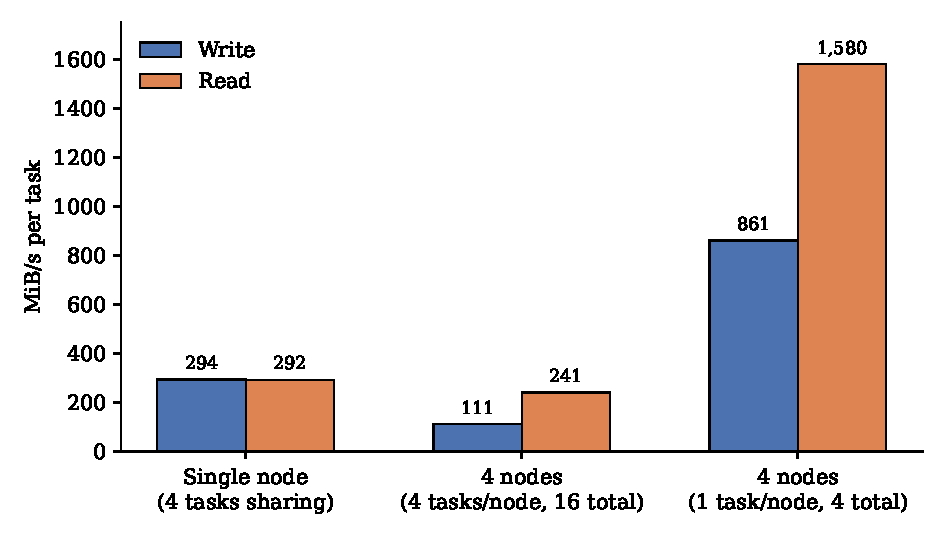
\includegraphics[width=0.85\textwidth]{placement_chart.pdf}
\end{center}

Per-task throughput with one task isolated per node is three to eight times higher than either configuration where tasks share a node. This is the most notable finding in this POC. It suggests same-node contention, most likely local TCP stack and page cache pressure from co-located tasks, costs substantially more per-task throughput than crossing the network to a different node.

This comparison is not a clean single-variable test. The single-node run held 16 GB of aggregate working set on one node; the isolated run held 4 GB spread across four nodes. Concurrency and per-node data volume both changed at once, so this result should be read as ``spread out and lightly loaded clearly outperforms concentrated and busy,'' not as an isolated measurement of network cost alone. A follow-up run holding total data volume and task count constant while only changing placement (for example, 4 tasks on 1 node with a 4 GB total working set, against 4 tasks on 4 different nodes with the same 4 GB total) would isolate the network variable cleanly.

\subsection*{Metadata (mdtest, single node, 4 tasks, 4000 files)}

\begin{center}
\begin{tabular}{lr}
\toprule
Operation & Rate (ops/sec) \\
\midrule
File creation & 7{,}000 \\
File stat & 153{,}876 \\
File read & 124{,}328 \\
File removal & 14{,}154 \\
Tree creation & 687 \\
Tree removal & 289 \\
\bottomrule
\end{tabular}
\end{center}

This is a first, conservative-scale metadata baseline. File count was kept low deliberately for this initial pass; a larger run is a reasonable next step once this baseline is reviewed.

\section*{Observations}

\begin{enumerate}
\item \textbf{A real baseline now exists where none did before.} RTS's operating assumption that GPFS-over-TCP performs adequately was previously untested. These numbers give a concrete reference point for that judgment and for any future comparison against verbs.

\item \textbf{Per-task contention on a shared node appears to be a bigger factor than network transport.} The three- to eight-fold per-task throughput difference between isolated and co-located placement is large enough to be operationally relevant independent of the TCP-versus-verbs question. If this holds up under a cleaner controlled test, it has implications for how multi-task jobs are best scheduled onto scratch-heavy workloads, not just for the fabric question this POC originally set out to inform.

\item \textbf{Two infrastructure gaps surfaced as a byproduct of getting this POC running, both worth independent tickets:}
\begin{itemize}
\item \texttt{openmpi/gcc/64/4.1.6} in the module tree has no bundled \texttt{libpmix.so} and cannot launch any MPI job. The working alternative at \texttt{/usr/mpi/gcc/openmpi-4.1.7a1} is not exposed through Lmod and was most likely built by someone on RTS working around module-tree incompleteness, not delivered by a vendor, though its provenance is not confirmed.
\item That same vendor MPI's CPU-binding logic fails outright under Slurm's cgroup-restricted CPU sets and requires \texttt{--bind-to none} on every launch. This did not matter for an I/O benchmark but would matter for a compute-bound MPI code.
\end{itemize}

\item \textbf{Tooling is built to be reused, not just this once.} The benchmark scripts, parser, and CSV output are structured to be re-run on a monthly cadence or after fabric and GPFS changes, building a trend line rather than a single snapshot. Output is also structured for eventual Zabbix ingestion alongside the existing fabric error-counter monitoring work, though that ingestion is not yet wired to a live server.
\end{enumerate}

\section*{Suggested Next Steps}

\begin{enumerate}
\item Review these numbers and decide whether they change or confirm the current TCP-over-verbs posture.
\item If the per-task placement effect seems worth pursuing, run the controlled comparison described above (constant task count and data volume, placement as the only variable).
\item Scale up the mdtest file count for a more representative metadata baseline.
\item Consider a verbs-enabled comparison run on a small cordoned-off node subset, now that a TCP baseline exists to compare it against.
\end{enumerate}

\end{document}

